\documentclass[10pt,a4paper,notitlepage]{article}
\usepackage{amssymb}
\usepackage{amsthm}
\usepackage{amsmath}
\usepackage{array}
\usepackage{caption}
\usepackage{color}
\usepackage{enumitem}
\usepackage{fancyhdr}
\usepackage{fancyvrb}
\usepackage{letltxmacro}
\usepackage{graphicx}
\usepackage{subcaption}
\usepackage[usenames,dvipsnames]{xcolor}
\usepackage{tikz}
\usetikzlibrary{%
  arrows,%
  shapes.misc,% wg. rounded rectangle
  shapes.arrows,%
  chains,%
  matrix,%
  positioning,% wg. " of "
  scopes,%
  decorations.pathmorphing,% /pgf/decoration/random steps | erste Graphik
  shadows%
}
\usepackage{tkz-graph}
\renewcommand*{\EdgeLineWidth}{0.15pt}
\usepackage{polynom}
\usepackage{hyperref}
\usepackage{listings}
\setlength{\baselineskip}{16.0pt}
\setlength{\parskip}{3pt plus 2pt}
\setlength{\parindent}{20pt}
\setlength{\oddsidemargin}{0cm}
\setlength{\evensidemargin}{0cm}
\setlength{\marginparsep}{0cm}
\setlength{\marginparwidth}{0cm}
\setlength{\marginparpush}{0cm}
\setlength{\textwidth}{162mm}
\setlength{\headsep}{0.15in}
\pagestyle{fancy}

%%--! Custom Python listings configuration, courtesy of redmode on TeX StackExchange: http://tex.stackexchange.com/questions/83882/how-to-highlight-python-syntax-in-latex-listings-lstinputlistings-command/#83883
\usepackage{listings}

% Default fixed font does not support bold face
\DeclareFixedFont{\ttb}{T1}{txtt}{bx}{n}{12} % for bold
\DeclareFixedFont{\ttm}{T1}{txtt}{m}{n}{12}  % for normal

% Custom colors
\usepackage{color}
\definecolor{deepblue}{rgb}{0,0,0.5}
\definecolor{deepred}{rgb}{0.6,0,0}
\definecolor{deepgreen}{rgb}{0,0.5,0}

% Python style for highlighting
\newcommand\pythonstyle{
  \lstset{
    language=Python,
    basicstyle=\ttm\small,
    % Add keywords here
    otherkeywords={self, None},
    keywordstyle=\ttb\small\color{deepblue},
    % Custom highlighting
    emph={relax_query,
          _generate_sample_data,
          _extract_rules,
          rul_distance},
    % Custom highlighting style
    emphstyle=\ttb\small\color{deepred},
    stringstyle=\color{deepgreen},
    % Any extra options here
    frame=tb,
    showstringspaces=false
  }
}


% Python environment
\lstnewenvironment{python}[1][]
{
  \pythonstyle
  \lstset{#1}
}
{}

% Python for external files
\newcommand\pythonexternal[2][]
{
  {
    \pythonstyle
    \lstinputlisting[#1]{#2}
  }
}

% Python for inline
\newcommand\pythoninline[1]{{\pythonstyle\lstinline!#1!}}
%%--! End of redmode's custom Python listings configuration.

\newcommand\tttilde[0]{{\raise.17ex\hbox{$\scriptstyle\mathtt{\sim}$}}}

\newcommand\ttscore[0]{\underline{\hspace{0.2cm}}}

\lhead{\footnotesize \parbox{11cm}{UNC Charlotte} }
\chead{\footnotesize Parse GO Documentation}
\rhead{\footnotesize Christian Gibson}
\begin{document}

The methods provided in the \texttt{parse\ttscore go} module allow for the creation of objects through which the Gene Ontology can be accessed programmatically. Currently, the module contains one object definition; \texttt{parse\ttscore obo}, which is capable of interpreting the Gene Ontology in the OBO flat-file format. Object instantiation accepts the following parameters:

\noindent \begin{tabular}{|c|p{5.22in}|} \hline
  \texttt{weights} &
  A dictionary object which serves to map relations within the Gene Ontology to weights based off of how much the user wants to restrict movement along a given relation when reducing a list of GO terms. If a given relation is not included in the dictionary, then that relation is ignored entirely. The value of a weight is meaningless in of itself, and is used solely in order to score different paths, where a larger score represents a longer path. As an example, given the weight dictionary \texttt{\{"is\ttscore a":1, "part\ttscore of":3\}}, a path that consists of three consecutive ``is\ttscore a" relations will be treated as if it is the same length as a path that consists of a single ``part\ttscore of" relation. Currently, this dictionary defaults to \texttt{\{"is\ttscore a":\ 1, "part\ttscore of":\ 2, "regulates":\ 5\}}.
  \\ \hline
  \texttt{roots} &
  The list of GO terms that serve to root the ontology in general. As of the time of writing, this list defaults to the GO terms ``GO:0003674", ``GO:0005575", and ``GO:0008150".
  \\ \hline
  \texttt{relations} &
  The list of relations found in the Gene Ontology. As of the time of writing, this list defaults to ``is\ttscore a", ``part\ttscore of", ``regulates", ``negatively\ttscore regulates", ``positively\ttscore regulates", ``has\ttscore part", ``occurs\ttscore in", and ``happens\ttscore during".
  \\ \hline
  \texttt{disjoint} &
  The list of relations that, when used to build a directed graph from the Gene Ontology, result in an acyclic graph. As of the time of writing, the sole relation in the Gene Ontology that meets this requirement is the ``is\ttscore a" relation.
  \\ \hline
  \texttt{source\ttscore path} &
  The filesystem path that points to the Gene Ontology OBO dump. If not provided, the script looks inside its own directory for a file entitled \texttt{go.obo}. If none is found, it attempts to download one from \url{http://geneontology.org/ontology/go.obo}.
  \\ \hline
  \texttt{save\ttscore detail} &
  A boolean flag that, when set to \texttt{True}, creates an internal dictionary \texttt{obo\ttscore detail} that contains all information corresponding to a given GO term found in the original Gene Ontology OBO dump.
  \\ \hline
  \texttt{verbose} &
  A boolean flag that, when set to \texttt{True}, will result in the object printing debug information during method calls.
  \\ \hline
\end{tabular}\\

Following object instantiation, the following methods can be called, with the caveat that each method's output can vary wildly based off of what values were passed to each function parameter when the original \texttt{parse\ttscore obo} object was created.

\texttt{find\ttscore lsca(go\ttscore term1, go\ttscore term2)}:\\
Central to the GO term set reduction functionality of the \texttt{parse\ttscore obo} object is the \texttt{find\ttscore lsca} method. When provided with two GO terms, the \texttt{find\ttscore lsca} method attempts to find the Lowest Single Common Ancestor \footnote{Johannes Fischer, Daniel H. Huson, New common ancestor problems in trees and directed acyclic graphs, Information Processing Letters, Volume 110, Issues 8–9, 1 April 2010, Pages 331-335, ISSN 0020-0190, http://dx.doi.org/10.1016/j.ipl.2010.02.014.
(\url{http://www.sciencedirect.com/science/article/pii/S0020019010000487})} (abbreviated as LSCA) between the two GO terms. This method starts by locating the root term within \texttt{roots} that minimalizes the summed squared distance from both GO terms. If such a shared root is located, then we compute the list of all reachable terms for each of the two GO terms, and compute the intersection of these two term sets. At this point, the set intersection contains at least the shared root we found originally. For each GO term in the resulting intersection, we calculate the summed squared distance from that GO term to each of the two GO terms, as well as the distance between that GO term and the shared root term. Finally, we select the GO term from this intersection with the greatest distance from the shared root term, and that which minimizes the distance from the two original GO terms. This term is then labeled the LSCA between the two original GO terms. As a visual example, the selection process proceeds as follows:

\begin{center}
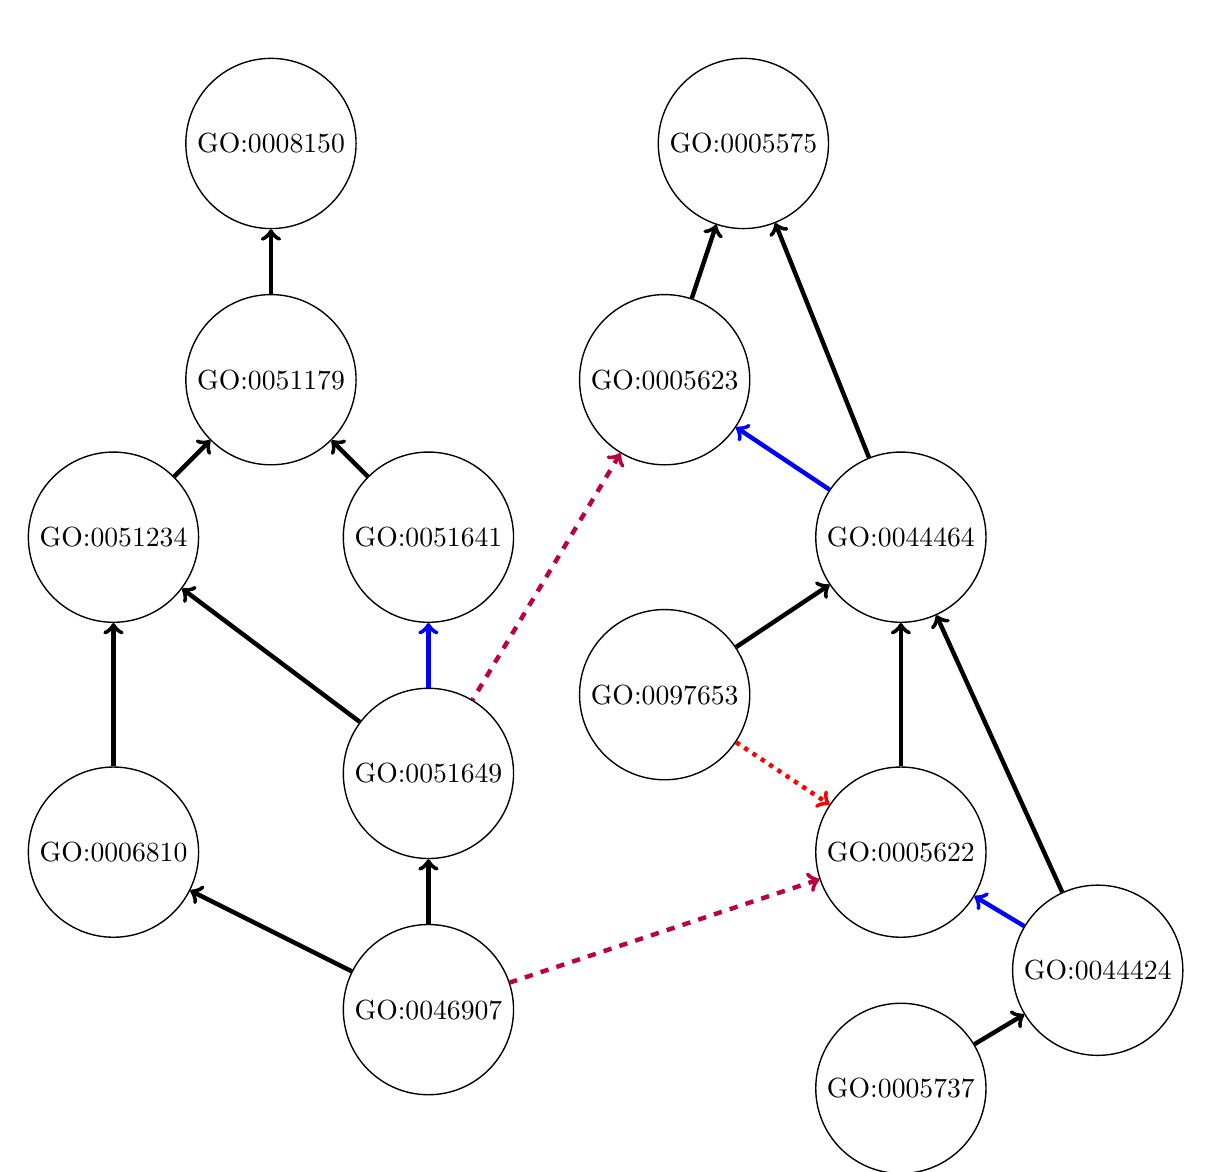
\begin{tikzpicture}
  \GraphInit[vstyle=Normal]
  \Vertex[L=GO:0008150, x= -3.0, y=  0.0]{08150}
  \Vertex[L=GO:0051179, x= -3.0, y= -3.0]{51179}
  \Vertex[L=GO:0051234, x= -5.0, y= -5.0]{51234}
  \Vertex[L=GO:0051641, x= -1.0, y= -5.0]{51641}
  \Vertex[L=GO:0006810, x= -5.0, y= -9.0]{06810}
  \Vertex[L=GO:0051649, x= -1.0, y= -8.0]{51649}
  \Vertex[L=GO:0046907, x= -1.0, y=-11.0]{46907}
  
  \Vertex[L=GO:0005575, x= +3.0, y=  0.0]{05575}
  \Vertex[L=GO:0005623, x= +2.0, y= -3.0]{05623}
  \Vertex[L=GO:0044464, x= +5.0, y= -5.0]{44464}
  \Vertex[L=GO:0097653, x= +2.0, y= -7.0]{97653}
  \Vertex[L=GO:0005622, x= +5.0, y= -9.0]{05622}
  \Vertex[L=GO:0044424, x= +7.5, y=-10.5]{44424}
  \Vertex[L=GO:0005737, x= +5.0, y=-12.0]{05737}
  
  % "is_a" relations
  \tikzset{EdgeStyle/.style = {<-, ultra thick, black}}
  \Edge(08150)(51179)
  \Edge(51179)(51234)
  \Edge(51179)(51641)
  \Edge(51234)(51649)
  \Edge(06810)(46907)
  \Edge(51649)(46907)
  \Edge(51234)(06810)
  \Edge(05575)(05623)
  \Edge(05575)(44464)
  \Edge(44464)(97653)
  \Edge(44424)(05737)
  \Edge(44464)(44424)
  \Edge(44464)(05622)
  
  % "part_of" relations
  \tikzset{EdgeStyle/.style = {<-, ultra thick, blue}}
  \Edge(51641)(51649)
  \Edge(05622)(44424)
  \Edge(05623)(44464)
  
  % "occurs_in" relations
  \tikzset{EdgeStyle/.style = {<-, dashed, ultra thick, purple}}
  \Edge(05623)(51649)
  \Edge(05622)(46907)
  
  % "has_part" relations
  \tikzset{EdgeStyle/.style = {->, ultra thick, dotted, red}}
  \Edge(97653)(05622)
\end{tikzpicture}
\end{center}

Provided in the above visual is a subsection of the Gene Ontology; in particular, it contains all nodes that can be reached from GO:0005737 (cytoplasm) or from GO:0046907 (intracellular transport). It contains four types of relations: the \texttt{"is\ttscore a"} relation, denoted by a black arrow, the \texttt{"part\ttscore of"} relation, denoted by a blue arrow, the \texttt{"occurs\ttscore in"} relation, denoted by a dashed, purple arrow, and finally the \texttt{"has\ttscore part"} relation, denoted by a dotted, red arrow. The process for finding the LSCA between GO:0005737 and GO:0046907 then occurs as follows:

\begin{enumerate}[nolistsep]
  \item Locate the shared root: in this case, GO:0005575.
  \item Determine list of all reachable GO terms from either term:
  \begin{enumerate}[nolistsep]
    \item \textit{GO:0005737}: GO:0044424, \textbf{GO:0005622}, \textbf{GO:0044464}, \textbf{GO:0005623}, \textbf{GO:0005575}.
    \item \textit{GO:0046907}: GO:0006810, GO:0051649, \textbf{GO:0005622}, GO:0051234, GO:0051641, \textbf{GO:0044464}, GO:0051179, \textbf{GO:0005623}, GO:0008150, \textbf{GO:0005575}.
  \end{enumerate}
  \item Determine list of shared terms: \textbf{GO:0005622}, \textbf{GO:0044464}, \textbf{GO:0005623}, \textbf{GO:0005575}.
  \item Determine which term is furthest from the shared root: \textbf{GO:0005622} (intercellular).
  \item As we only have one term, it is our LSCA. If there were more, the term with the smallest summed squared distance from both GO:0005737 and GO:0046907 would be selected as our LSCA.
\end{enumerate}

\texttt{reduce\ttscore list(go\ttscore terms, branch\ttscore count, avoid\ttscore roots, range\ttscore modifier, range\ttscore width,}\\ \smallskip
\texttt{\ \ \ \ \ \ \ \ \ \ \ \ \ \ \ \ path\ttscore lengths, dijkstra\ttscore lengths, verbose)}:\\

\pagebreak

\texttt{fetch\ttscore update(url, filepath)}:

\noindent \begin{tabular}{|c|p{5.45in}|} \hline
  \texttt{url} &
  The full URL from which to fetch an updated version of \texttt{go.obo}. If none is provided, it defaults to \url{http://geneontology.org/ontology/go.obo}. \\ \hline
  \texttt{filepath} &
  The full or relative system path where the downloaded file should be saved. If none is provided, it defaults to \texttt{./go.obo}. \\ \hline
\end{tabular}\\
Method used to update the base \texttt{go.obo} file that the \texttt{parse\ttscore obo} relies on when building its internal graph representation of the Gene Ontology.

\smallskip

\texttt{generate\ttscore detail()}:\\
Simple method that allows the user to create the \texttt{obo\ttscore detail} object if they set the \texttt{save\ttscore detail} flag to \texttt{False} during object instantiation without having to recreate the entire \texttt{parse\ttscore obo} object.

\smallskip

\texttt{generate\ttscore circle\ttscore representation(size, verbose)}:

\noindent \begin{tabular}{|c|p{5.4in}|} \hline
  \texttt{size} &
  An integer value that defines the side length of a square that could contain the entirety of the generated representation. Defaults to $960$, which can result in the placement of terms anywhere between the cartesian coordinate point $(-480,-480)$ and $(480,480)$. \\ \hline
  \texttt{verbose} &
  A boolean flag that, when set to \texttt{True}, will result in the method printing debug information during the function's runtime. \\ \hline
\end{tabular}\\
An as of yet unimplemented method intended to provide cartesian coordinate points for each term found in the Gene Ontology such that a roughly circular representation of the overall Gene Ontology can be constructed by associating each term with its matching $(x,y)$ coordinate.
\end{document}